
%(BEGIN_QUESTION)
% Copyright 2015, Tony R. Kuphaldt, released under the Creative Commons Attribution License (v 1.0)
% This means you may do almost anything with this work of mine, so long as you give me proper credit

Read and outline the introduction to the ``Safety Instrumented Functions and Systems'' section of the ``Process Safety and Instrumentation'' chapter in your {\it Lessons In Industrial Instrumentation} textbook.  Note the page numbers where important illustrations, photographs, equations, tables, and other relevant details are found.  Prepare to thoughtfully discuss with your instructor and classmates the concepts and examples explored in this reading.

\underbar{file i04646}
%(END_QUESTION)





%(BEGIN_ANSWER)


%(END_ANSWER)





%(BEGIN_NOTES)

\noindent
{\bf SIF} = one or more components designed to implement a specific safety function.

\vskip 10pt

\noindent
{\bf SIS} = collection of SIFs designed to bring a process to a safe condition in the event of multiple types of failures.

\vskip 10pt

The balance between dependability and security is very important.  It is possible to make a process so ``paranoid'' that it shuts down needlessly.  

\vskip 10pt

Two series block valves on a pipeline increases dependability (dependability., but decreases security (i.e. increases chance of needless shutdown).

\vskip 10pt

``MooN'' notation used to express number of elements essential for a function versus total number of elements.  Dual series block valves are 1oo2 for dependability but 2oo2 for security.  Another way of stating this is ``fault tolerance'' (i.e. how many elements can fail and still allow the system to perform its intended function).  Dual series block valves have a dependability fault tolerance of 1 and a security fault tolerance of 0.

Parallel block valves on a pipeline are 2oo2 for dependability and 1oo2 for security.  In other words, this system has a dependability fault tolerance of 0 and a security fault tolerance of 1.

\vskip 10pt

When analyzing systems with lots of redundant components, it is important to consider the number of those components which {\it must} function in order to fulfill the stated purpose.  The four-valve system shown in the book is actually 3oo4, not 2oo4, because we need at least three of the valves to properly function in order to {\it guarantee} the desired result.  Having just two function might not be enough if they're the wrong two!

\vskip 10pt

Sensors used in safety instrumented systems are always independent of sensors used for regulatory control, so that we avoid common-cause failure modes (e.g. a failure on one sensor causing both the regulatory controls and the safety shutdown system to fail).

Continuous sensors are preferred for SIS over discrete sensors (i.e. process switches) because their signals give useful diagnostic information.  Redundant process transmitters are common in SIS where a very high level of reliability is needed.  Signal-selector functions called {\it voting} modules are used to select from multiple redundant transmitter signals, with high and low selection providing 1oo3 dependability and median providing 2oo3 dependability.

\vskip 10pt

SIS controllers must be separate from regulatory control systems, in honor of the same principle applied to SIS sensors.  These go by the name of {\it logic solver} rather than ``controller'' and usually take the form of a special PLC (sometimes called a ``safety PLC'').  Logic solvers themselves are designed to exhibit unusually high reliability, often with redundant processors.  Rockwell's {\it GuardLogix} system, for example, provide special instructions for monitoring dual-redundant discrete inputs from process switches.  Triple redundancy is commonly seen in logic solvers, for example those manufactured by Triconex and ICS-Triplex where not only the processors are triple-redundant but also the signal conditioning circuitry and communication channels between components.

\vskip 10pt

SIS final control elements are also often separate from regulatory final control elements.  {\it Chopper valves} are special on/off valves designed specifically for safety shutdown function and not for regulatory control.  In some cases it is acceptable to augment the regulatory control valve with a special solenoid designed to override its operation in the event of an abnormal (shutdown) condition.

Final control elements are the most failure-prone component of an SIS, and they are also the most expensive.  One way to minimize cost while increasing reliability is to use a single valve for safety shutdown but to periodically stroke-test that valve to ensure its dependability.  A {\it partial stroke test} involves moving the safety shutdown valve partially to ensure it isn't frozen in position (failed), while still allowing normal operation to continue.





\vskip 20pt \vbox{\hrule \hbox{\strut \vrule{} {\bf Suggestions for Socratic discussion} \vrule} \hrule}

\begin{itemize}
\item{} Contrast {\it dependability} versus {\it security} in a complex system.
\item{} Explain why two different shutoff valve technologies are shown in the double-block pipeline valve system.
\item{} Suppose a set of three redundant temperature sensors monitors the temperature of an industrial furnace.  The furnace will shut down if any of the three sensors detects an abnormally high temperature.  
\itemitem{} Determine the MooN rating for dependability.  
\itemitem{} Determine the MooN rating for security.
\itemitem{} Determine the fault tolerance for dependability.
\itemitem{} Determine the fault tolerance for security.
\item{} Suppose a set of three redundant temperature sensors monitors the temperature of an industrial furnace.  The furnace will shut down only if all three of the sensors detect an abnormally high temperature.  
\itemitem{} Determine the MooN rating for dependability.  
\itemitem{} Determine the MooN rating for security.
\itemitem{} Determine the fault tolerance for dependability.
\itemitem{} Determine the fault tolerance for security.
\item{} Suppose a set of three redundant temperature sensors monitors the temperature of an industrial furnace.  The furnace will shut down if two out of the three sensors detect an abnormally high temperature.  
\itemitem{} Determine the MooN rating for dependability.  
\itemitem{} Determine the MooN rating for security.
\itemitem{} Determine the fault tolerance for dependability.
\itemitem{} Determine the fault tolerance for security.
%\item{} Explain how the logic solver (safety PLC) in an SIS differs from a regular control system.
%\item{} Explain what a {\it chopper valve} is and where we might find one used.
%\item{} Explain what {\it partial stroke testing} is and why we do it for SIS final control elements.
\medskip











\vfil \eject

\noindent
{\bf Prep Quiz:}

Identify the reason why two {\it different kinds} of blocks valves are used in this high-reliability valve system:

$$\includegraphics[width=15.5cm]{i04646x01.eps}$$

\begin{itemize}
\item{} Different valve designs reduces maintenance costs
\vskip 5pt 
\item{} Identical valve designs would increase system construction cost
\vskip 5pt 
\item{} Two motor-actuated valves would increase risk of sparks (explosion)
\vskip 5pt 
\item{} Fluid throttling is quieter using different valves in series
\vskip 5pt 
\item{} Different valve designs reduces the risk of common-cause failures
\vskip 5pt 
\item{} The engineer couldn't decide between two different valve vendors
\end{itemize}

%INDEX% Reading assignment: Lessons In Industrial Instrumentation, process dependability.(SIS intro)

%(END_NOTES)

